\documentclass{article}
\usepackage[letterpaper, margin=1in]{geometry}
\usepackage{fancyhdr}
\usepackage[utf8]{inputenc}
\usepackage{amsmath}
\usepackage{circuitikz}
\usepackage{pgfplots}
\usepackage{bm}
\usepackage{amsfonts}
\usepackage{graphicx}
\usepackage{float}
\usepackage{subcaption}
\usepackage[dvipsnames]{xcolor}
\usepackage{array}
\usepackage[colorlinks=true, allcolors=blue]{hyperref}
\title{6. Complex Power in AC Circuits \\  \large Introduction to Electric Circuits \\ Supplemental Instruction}
\author{Cooper McAllister}
\date{April 16 2026}
\begin{document}
\fancypagestyle{footerstyle} {
	\fancyhf{}
	\renewcommand{\headrulewidth}{0pt}
	\renewcommand{\footrulewidth}{0.4pt}
	\fancyfoot[L]{\textit{For personal study and students leading supplemental instruction, \\ with attribution given to the author. \\ Find more at coopermcallister.com}}
	\fancyfoot[R]{\thepage}
}
\pagestyle{footerstyle}
\maketitle
\thispagestyle{footerstyle}

\begin{center}
\textit{This document is not a substitute for a textbook or classroom instruction. It may contain errors and is intended to be used only to the extent that it is helpful to supplement students' learning experience.}
\end{center}

\section{Introduction}


\section{RMS Values}
When we analyze the power of AC circuits, we use \textbf{RMS values}, which give the effective value of a sinusoidal voltage or current. For a sinusoidal voltage $\bm{V} = V_m \angle \alpha_v$ or current $\bm{I} = I_m \angle \alpha_i$, the RMS value is
$$V_{rms} = \frac{V_m}{\sqrt{2}} \qquad I_{rms} = \frac{I_m}{\sqrt{2}}$$


\section{Average (True) Power}
For a component or network, given $\bm{V} = V_m \angle \alpha_v$ and $\bm{I} = I_m \angle \alpha_i$, the \textbf{average power} is:
$$P = V_{rms}I_{rms}\cos(\alpha_v - \alpha_i)$$
Or, using magnitudes,
$$P = \frac{V_mI_m}{2}\cos(\alpha_v - \alpha_i)$$
Average power is sometimes also called \textbf{true power} or \textbf{real power}. The \textbf{unit} of average power is Watts (W). Average power is associated with resistance.

\section{Reactive Power}
For a component or network, given $\bm{V} = V_m \angle \alpha_v$ and $\bm{I} = I_m \angle \alpha_i$, the \textbf{reactive power} is:
$$Q = V_{rms}I_{rms}\sin(\alpha_v - \alpha_i)$$
Or, using magnitudes,
$$Q = \frac{V_mI_m}{2}\sin(\alpha_v - \alpha_i)$$
The \textbf{unit} of average power is Volt Amps Reactive (VAR). Reactive power is associated with reactive components (inductors and capacitors).

\section{Apparent Power}
For a component or network, given $\bm{V} = V_m \angle \alpha_v$ and $\bm{I} = I_m \angle \alpha_i$, the \textbf{apparent power} is:
$$S = V_{rms}I_{rms}$$
Or, using magnitudes,
$$S = \frac{V_mI_m}{2}$$
The \textbf{unit} of apparent power is Volt Amps (VA).

\section{Power Factor}
For a component or network, given $\bm{V} = V_m \angle \alpha_v$ and $\bm{I} = I_m \angle \alpha_i$, the \textbf{power factor} is:
$$PF = \cos(\alpha_v - \alpha_i)$$
Power factor is specified as either leading or lagging, describing whether the current leads or lags the voltage. If $\alpha_i > \alpha_v$, the power factor is leading; if $\alpha_i < \alpha_v$, the power factor is lagging.

\section{Complex Power and the Power Triangle}
In summary, we have
$$P = V_{rms}I_{rms}\cos(\alpha_v - \alpha_i)$$
$$Q = V_{rms}I_{rms}\sin(\alpha_v - \alpha_i)$$
$$S = V_{rms}I_{rms}$$
$$PF = \cos(\alpha_v - \alpha_i)$$
Complex power is
$$\bm{S} = P + jQ = S \angle (\alpha_v - \alpha_i)$$
We can draw this as a triangle in the complex plane, where average power is the horizontal component, reactive power is the vertical component, and apparent power is the magnitude:
\begin{figure}[H]
\centering
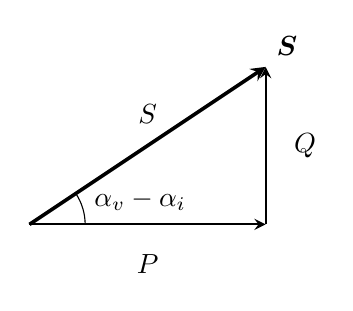
\begin{tikzpicture}
\draw[line width=1.3pt,-stealth] (0, 0) -- (3, 2) node[anchor = south west] {$\bm{S}$};
\draw (1.5, 1.4) node[]{$S$};
\draw[line width=0.8pt,-stealth] (0, 0) -- (3, 0);
\draw (1.5, -0.5) node[]{$P$};
\draw[line width=0.8pt,-stealth] (3, 0) -- (3, 2);
\draw (3.5, 1) node[]{$Q$};
\draw (0.707,0) arc (0:33.69:0.707);
\draw (0.7, 0.3) node[anchor = west]{$\alpha_v - \alpha_i$};
\end{tikzpicture}
\end{figure}


\newpage
\section*{References}
\begin{itemize}
\item M. Iordache. Class Lectures, Topic: ``Electric circuits.'' EEGR 2053, School of Engineering and Engineering Technology, LeTourneau University, 2025.
\item M. Iordache. 2024. EEGR 2053 Electric circuits [PowerPoint slides]. Available: \\ https://mviordache.name/EEGR2053/index.html
\item T. L. Floyd and D. M. Buchla, Principles of Electric Circuits: Conventional Current, 10th ed. Hoboken, NJ: Pearson Education, 2020.
\item O. Ortiz. 2025. ENGR 2053 Intro to electric circuits [PowerPoint slides].
\end{itemize}

	
\end{document}